\section{Lateral movement}

\begin{figure}
  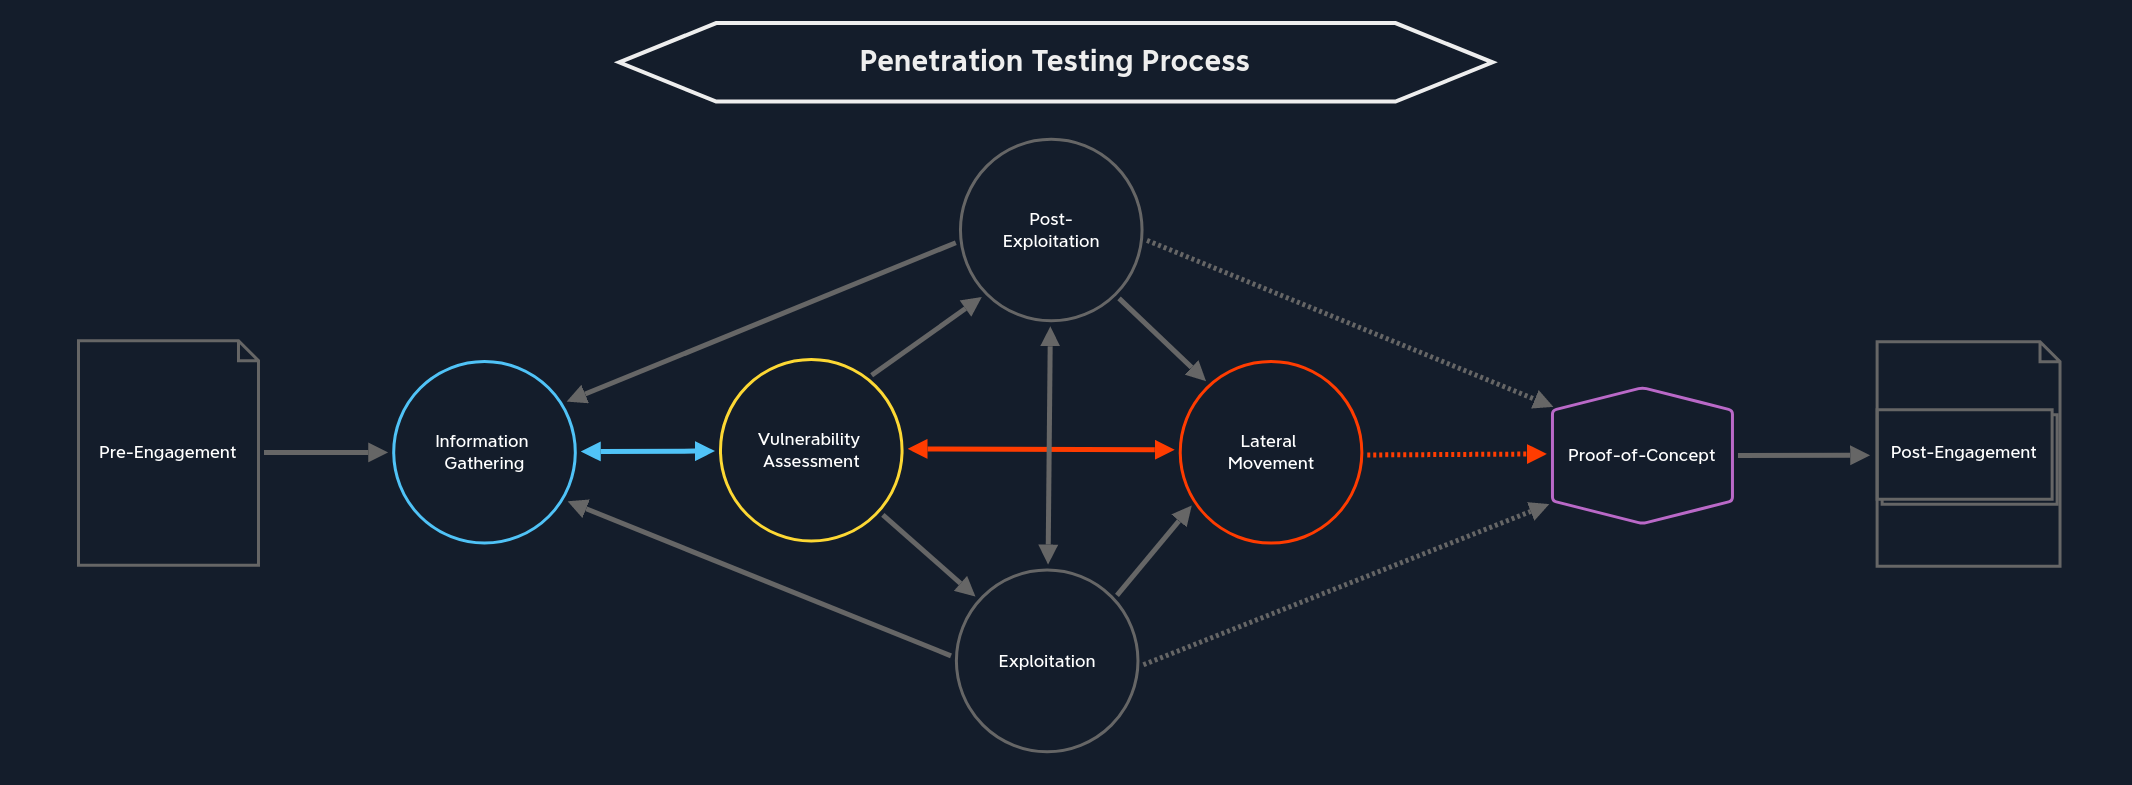
\includegraphics[width=\linewidth]{intro/process/images/lateral.png}
  \caption{Lateral movement}
  \label{fig:pentest-process-lateral}
\end{figure}

The goal here is that we test what an attacker could do within the entire
network. After all, the main goal is not only to successfully exploit a
publicly available system but also to get sensitive data or find all ways that
an attacker could render the network unusable. One of the most common examples
is ransomware. If a system in the corporate network is infected with
ransomware, it can spread across the entire network. It locks down all the
systems using various encryption methods, making them unusable for the whole
company until a decryption key is entered.

In the most common cases, the company is financially extorted to make a profit.
Often, it is only at this moment that companies realize how important IT
security is. If they had had a good penetration tester who had tested things
(and proper processes and layered defenses in place), they probably could have
prevented such a situation and the financial (if not legal) damage. It is often
forgotten that in many countries, the CEOs are held liable for not securing
their customer data appropriately.

In this stage, we want to test how far we can move manually in the entire network and what vulnerabilities we can find from the internal perspective that might be exploited. In doing so, we will again run through several phases:
\begin{itemize}
    \item  Pivoting
    \item  Evasive Testing
    \item  Information Gathering
    \item  Vulnerability Assessment
    \item  (Privilege) Exploitation
    \item  Post-Exploitation
\end{itemize}

As seen in the graphic above, we can move to this stage from the Exploitation and the Post-Exploitation stage. Sometimes we may not find a direct way to escalate our privileges on the target system itself, but we have ways to move around the network. This is where Lateral Movement comes into play.

\subsection{Pivoting}

In most cases, the system we use will not have the tools to enumerate the internal network efficiently. Some techniques allow us to use the exploited host as a proxy and perform all the scans from our attack machine or VM. In doing so, the exploited system represents and routes all our network requests sent from our attack machine to the internal network and its network components.

In this way, we make non-routable networks (and therefore publicly unreachable) can still be reached. This allows us to scan them for vulnerabilities and penetrate deeper into the network. This process is also known as Pivoting or Tunneling.

An elementary example could be that we have a printer at home that is not accessible from the Internet, but we can send print jobs from our home network. If one of the hosts on our home network has been compromised, it could be leveraged to send these jobs to the printer. Though this is a simple (an unlikely) example, it illustrates the goal of pivoting, which is to access inaccessible systems via an intermediary system.

\subsection{Evasive Testing}

Also, at this stage, we should consider whether evasive testing is part of the assessment scope. There are different procedures for each tactic, which support us in disguising these requests to not trigger an internal alarm among the administrators and the blue team.

There are many ways to protect against lateral movement, including network (micro) segmentation, threat monitoring, IPS/IDS, EDR, etc. To bypass these efficiently, we need to understand how they work and what they respond to. Then we can adapt and apply methods and strategies that help avoid detection.

\subsection{Information Gathering}

Before we target the internal network, we must first get an overview of which systems and how many can be reached from our system. This information may already be available to us from the last post-exploitation stage, where we took a closer look at the settings and configurations of the system.

We return to the Information Gathering stage, but this time, we do it from inside the network with a different view of it. Once we have discovered all hosts and servers, we can enumerate them individually.

\subsection{Vulnerability Assessment}

Vulnerability assessment from the inside of the network differs from the previous procedures. This is because far more errors occur inside a network than on hosts and servers exposed to the Internet. Here, the groups to which one has been assigned and the rights to different system components play an essential role. In addition, it is common for users to share information and documents and work on them together.

This type of information is of particular interest to us when planning our attacks. For example, if we compromise a user account assigned to a developer group, we may gain access to most of the resources used by company developers. This will likely provide us with crucial internal information about the systems and could help us to identify flaws or further our access.

\subsection{(Privilege) Exploitation}

Once we have found and prioritized these paths, we can jump to the step where we use these to access the other systems. We often find ways to crack passwords and hashes and gain higher privileges. Another standard method is to use our existing credentials on other systems. There will also be situations where we do not even have to crack the hashes but can use them directly. For example, we can use the tool Responder to intercept NTLMv2 hashes. If we can intercept a hash from an administrator, then we can use the pass-the-hash technique to log in as that administrator (in most cases) on multiple hosts and servers.

After all, the Lateral Movement stage aims to move through the internal network. Existing data and information can be versatile and often used in many ways.

\subsection{Post-Exploitation}

Once we have reached one or more hosts or servers, we go through the steps of the post-exploitation stage again for each system. Here we again collect system information, data from created users, and business information that can be presented as evidence. However, we must again consider how this different information must be handled and the rules defined around sensitive data in the contract.
